\chapter{Cyber Defence Matters}

\section{Exploratory Data Analysis of Cyberattacks}

In this chapter, an exploratory data analysis will be executed on cyber operations data from different sources, tracing trends, differences and insights that can be useful for the purpose of this research. One approach to assess the cyber defence strategies of the European Union members is to understand how those countries counter the attacks. Furthermore, it will help to recognise if the war in Ukraine had a direct effect on cyber operations in EU countries. 

\begin{figure}[H]
    \centering
    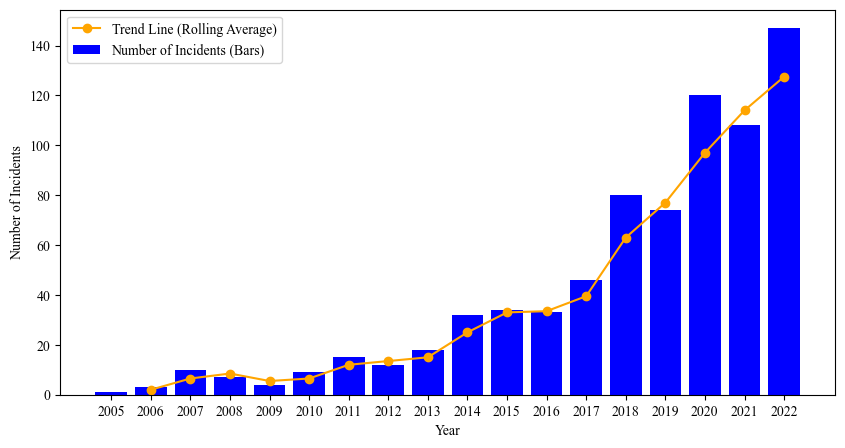
\includegraphics[width=1\textwidth]{Images/total_cyber.png}
    \caption{\textit{Total Cyber Operations from 2005 to 2022}}
    \source{Source: Cyber Operations Tracker}
    \label{total_cyber.png}
\end{figure}

As expected, in Figure \ref{total_cyber.png} the total number of cyber operations is constantly increasing. Noticeably, during the COVID-19 pandemic, we have experienced an increase of about 62.16\% of attacks compared to 2019. The surge in cyberattacks can be attributed significantly to the widespread adoption of remote work. This increase is primarily because individuals working from home lack the same level of inherent security and deterrent measures present in traditional office environments \parencite{nabe_2020_impact}. 

\begin{figure}[H]
    \centering
    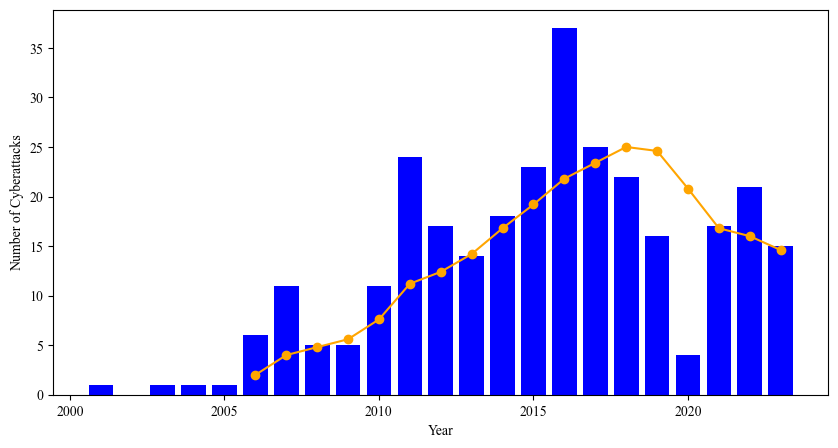
\includegraphics[width=1\textwidth]{Images/total_cyber_EU.png}
    \caption{\textit{Total Cyber Operations from 2000 to nowadays}}
    \source{Source:\autocite{eurepoc2023}
    \label{total_cyber_EU.png}
\end{figure}


However, it is important to note that the European context exhibits a decrease in recorded cyberattacks during the COVID-19 pandemic. These findings, as elucidated by the insights provided by Kerstin Zettl-Schabath, on behalf of the EuRepoC coding team, can be attributed to several factors. EuRepoC's approach to data collection differs from that of the Cyber Operations Tracker, which primarily focuses on politically motivated cyber incidents. According to Kerstin Zettl-Schabath \footnote{Kerstin Zettl-Schabath is part of the Coding Team of EuRepoC. The information was obtained through an exchange of emails.}, EuRepoC does not count non-politically motivated and fully disclosed cyberattacks in its database. Therefore, while it is true that overall cyberattacks increased during the pandemic, many of these attacks were more economically motivated and not necessarily politically driven. This fact underscores the importance of considering the motive and nature of cyber incidents when analysing the data.

Kerstin Zettl-Schabath provides several potential explanations for the discrepancy between EuRepoC's data and other sources:
\begin{enumerate}
    \item EuRepoC places particular emphasis on confirmed CIA (Confidentiality, Integrity, Availability) violations in their data collection. Some incidents recorded by other sources may be considered as \textit{attempted attacks} without confirmed CIA violations, leading to differences in reported incidents. It is essential to consider the criteria used by each database for assessing the intensity and impact of cyber incidents.
    \item EuRepoC's inclusion criteria do not cover genuine cybercrime cases that lack political or state involvement. This criterion was only added to their codebook in recent years. The rapid increase in non-politicized cybercrime incidents throughout the first year of the COVID-19 pandemic could account for part of the explanation for the lower incident count in EuRepoC's database compared to sources with different inclusion criteria.
    \item The assignment of incidents to a specific year can vary between databases based on criteria such as the actual start of the operation. This discrepancy may lead to differences in the reported number of incidents in a given year.
    \item Kerstin Zettl-Schabath also suggests a theoretical explanation related to the diversion of resources and capacities during the COVID-19 pandemic. The pandemic may have absorbed more resources at the state cyber level, leading to both fewer offensive cyber actions and fewer detections and attributions of incidents, which would have been relevant to EuRepoC's politically connoted inclusion criteria
\end{enumerate}

\begin{figure}[H]
    \centering
    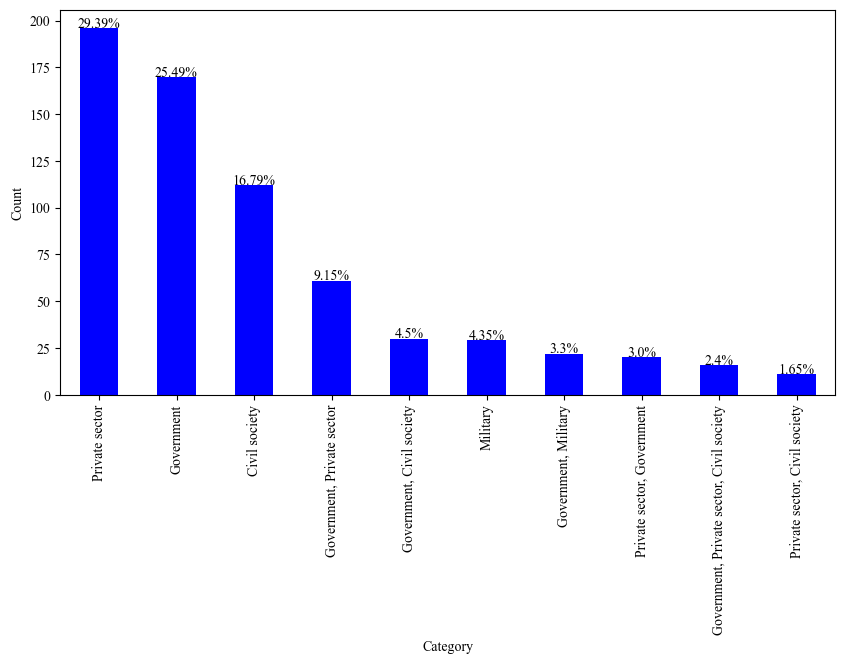
\includegraphics[width=\textwidth]{Images/top10sect.png}
    \caption{Top 10 Sectors Affected by Cyber Operations}
    \source{Source: Cyber Operations Tracker}
    \label{fig:top10sect}
\end{figure}

The categories most attacked are the private sector (29.35\%) and the government (25.22\%), while the military category constitutes 4.42\% of the worldwide cyber operations from 2005. Differently from the government and private sector, attacks on the military IT infrastructure are less disclosed while being at the same time difficult to be successful to its increase securitisation. 

\begin{figure}[H]
    \centering
    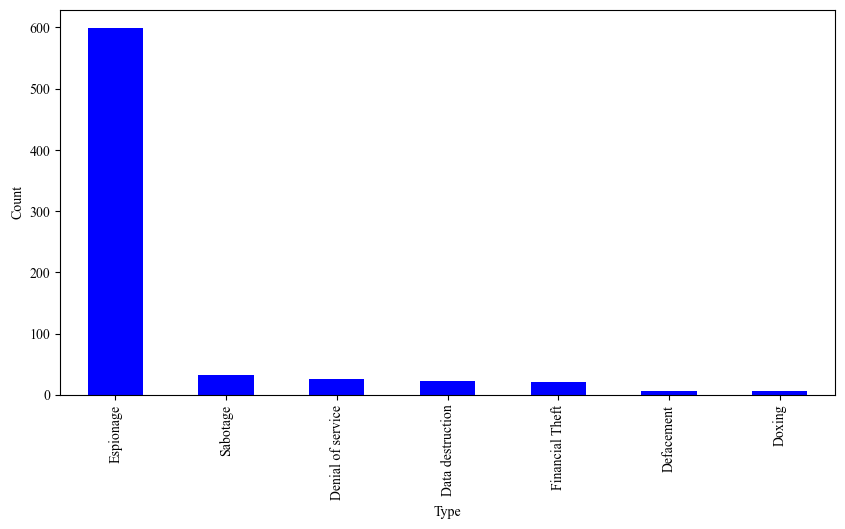
\includegraphics[width=\textwidth]{Images/top10type.png}
    \caption{Methods to conduct Cyber Operations}
    \source{Source: Cyber Operations Tracker}
    \label{fig:top10type}
\end{figure}

For what regards the goal of attacks, mainly relates to espionage. Cyber adversaries often seek to infiltrate both private sector and government networks to gather sensitive information, proprietary data, or state secrets. Espionage attacks aim to gain unauthorised access to critical data for intelligence purposes, economic advantage, or strategic planning. These attacks can have far-reaching consequences, ranging from compromising individual privacy to jeopardizing national security. 

\section{Why no destructive cyberattacks? }

Destruction-focused cyberattacks are relatively less common for several significant reasons. Firstly, these attacks often leave a more traceable trail of evidence, making it easier for cybersecurity experts to identify and attribute the source of the attack. Additionally, destructive cyberattacks can escalate conflicts and lead to severe real-world consequences, deterring some threat actors. Technical complexity and the need for deep knowledge of target vulnerabilities also make such attacks less attractive compared to data theft. Moreover, many cyberattacks are politically or strategically motivated, aiming to influence public opinion or cause economic disruption rather than physical destruction. International norms discourage destructive cyber operations and the cost-benefit analysis that cybercriminals and state-sponsored actors perform further contribute to their relative infrequency. While destructive cyberattacks are not unheard of, their risks and consequences make them a less common choice in the cyber threat landscape. 

On the other hand, for what regards the European context, the motive behind the attacks is mostly unknown. This is because cyberattacks are a major of the time part of operations that includes cyber, information and influence sphere with political objectives that are not specified with a blurred portrait as hybrid operations do. The EuRepoC use the codification from the Conflict Issues by the Conflict Barometer of the Heidelberg Institute for International Conflict Research (HIIK), to identify several cyber-conflict issues. 35\% of the issues relate to the system/ideology and international power conflicts. The first refers to change and/or influence in internal aspects of state affairs (socio-economic, legal, or political orientation). International power relates to changes in the relations of power in the international system or one of its regional systems \parencite{hiik_methodology}.

\begin{figure}[H]
    \centering
    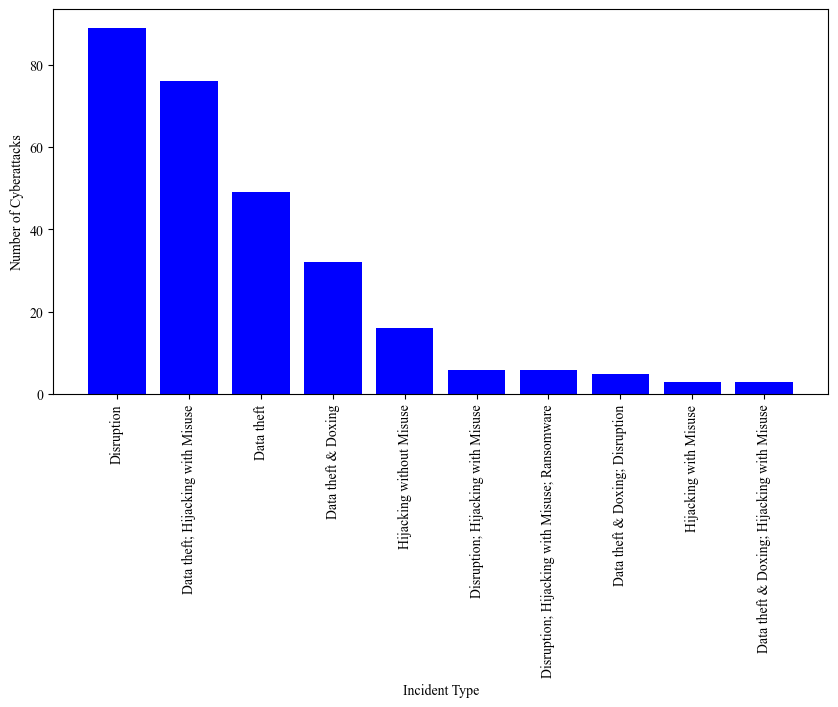
\includegraphics[width=\textwidth]{Images/eu_type.png}
    \caption{Classification of Cyber Operation in the EU by type}
    \source{Source:EuRepoC}
    \label{fig:eu_type}
\end{figure}

From 2001 to nowadays, the principal attack vectors for each of the modalities have evolved significantly. In the realm of disruption, attackers have increasingly employed distributed denial of service (DDoS) attacks, ransomware, and malware to disrupt critical systems and services. Meanwhile, in the domain of data theft, attackers have leveraged techniques such as phishing, social engineering, and advanced persistent threats (APTs) to gain unauthorized access to sensitive information and steal data. 

\section{Intensity of Cyber Operations}

The European countries have only in recent years given strategic importance to cyberspace and its security. Overall, the European countries were not able to handle the cyberattacks to avoid the disruptions, as Figure \ref{fig:avg} suggests. Firstly, there is a lack of sufficient infrastructure and investment to support the cybersecurity and cyberdefence policies and institutions in Europe \autocite{petratos_2014_cybersecurity}.  Additionally, the flexible and modern network technologies used by business organisations have opened the door for cybercriminals to initiate cyberattacks, leading to disruptions in the business process \autocite{sudar_2020_analysis}). The European Union also faces limitations as a cybersecurity actor, including its intergovernmental character and the lack of a collective vision on cyber-security among member states \autocite{sliwinski_2014_moving}


\begin{figure}[H]
    \centering
    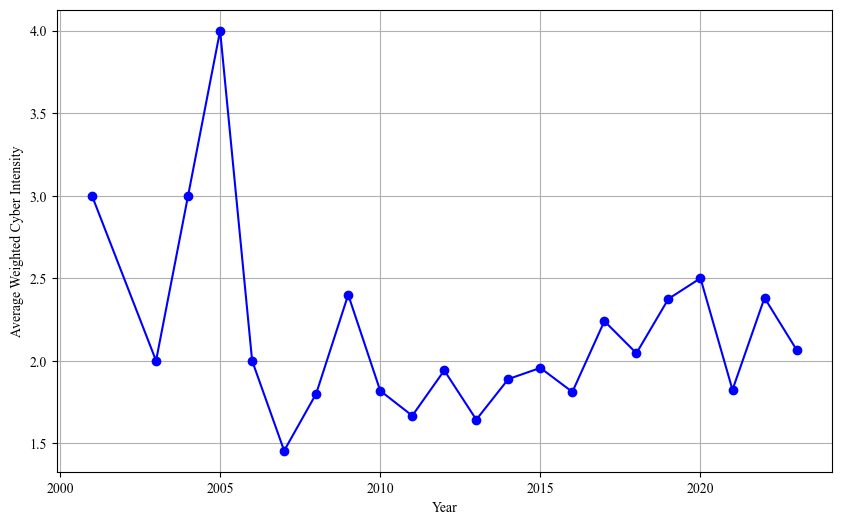
\includegraphics[width=\textwidth]{Images/avg.png}
    \caption{Average Weighted Cyber Intensity per Year in EU Countries}
    \source{Source:\autocite{eurepoc2023}}
    \label{fig:avg}
\end{figure}

For many different cyber incidents, the average cyber intensity has mostly remained low. Even in the case of the Estonia 2007 cyberattacks, where the EuRepoC acknowledged that the level of disruption was less severe than initially predicted, this pattern persisted. But it's important to remember that this incident still has political ramifications since it had a major influence on how NATO and the European Union would respond to state-sponsored cyberattacks.

On the other hand, some specific cyber incidents have displayed a noticeably high level of cyber intensity, such as the Ransomware House attack on the Hospital Clinic de Barcelona. Such incidents come into the high-intensity category, with a grade of 6 on the intensity scale, and are defined by their major interruption, probable data theft, system hijacking, and significant spatial and temporal consequences. The attack on Hospital Clinic de Barcelona serves as a sobering reminder of the changing and more advanced cyber risks critical infrastructure must contend with, particularly in the healthcare industry, where the stakes are very high.  

While the highest average in 2005 is associated with Poseidon, often referred to as the \textit{Poseidon Group}, which is a cyber espionage group known for its advanced and targeted attacks. Its activities primarily revolve around conducting cyber espionage campaigns against specific targets, with a particular focus on governmental and diplomatic entities, as well as critical infrastructure organizations. It was disclosed by Kaspersky in 2015 and has affected France, Russia, Brazil and United Stated among other countries\footnote{For more information: https://securelist.com/poseidon-group-a-targeted-attack-boutique-specializing-in-global-cyber-espionage/73673/}.
